\documentclass[11pt,letterpaper]{article}

\usepackage[margin=1in]{geometry}
\usepackage{graphicx}
\usepackage{subcaption}
\usepackage{booktabs}
\usepackage{hyperref}
\usepackage{parskip}
\usepackage{float}
\usepackage{microtype}
\usepackage{amsmath}

\hypersetup{colorlinks=true, linkcolor=blue, urlcolor=blue}

\title{\textbf{CS5330 Computer Vision -- Project 1}\\
       \large Image Manipulation and Video Filtering}
\author{Shriman Raghav Srinivasan \and Shyam Sreenivasan}
\date{May 2026}

\begin{document}

\maketitle

% ============================================================
\section*{Project Overview}
% ============================================================

For this project we built a live video filtering program in C++ using OpenCV.
The idea is that you run the program, point your webcam at something, and then
use different keys to switch between filters in real time. We implemented
filters for greyscale (two versions), sepia tone, Gaussian blur (two
implementations at different speeds), Sobel edge detection, gradient magnitude,
and a blur-and-quantize effect. We also integrated a face detector using a Haar
cascade and a depth estimation model called Depth Anything V2, which runs
through the ONNX runtime. On top of those, we added three custom effects:
color negative, emboss, and depth-based fog.

All the pixel manipulation functions are written from scratch in
\texttt{filter.cpp}. The main loop lives in \texttt{vidDisplay.cpp} and just
reads a frame, applies whatever filter is currently selected, and shows it. We
split the work: Shriman handled Tasks 4 through 9 (filters.cpp) and Shyam
handled the rest.

% ============================================================
\section*{Source Code}
% ============================================================

The full source code for this project is available at:\\
\url{https://github.com/shyams612/CS5330-Computer-Vision/tree/main/Projects/project1}

% ============================================================
\section*{Key Mapping}
% ============================================================

\begin{table}[H]
\centering
\begin{tabular}{clc}
\toprule
\textbf{Task} & \textbf{Description} & \textbf{Key} \\
\midrule
1   & Static image display             & -- \\
2   & Live color video                 & (default) \\
3   & OpenCV greyscale                 & \texttt{g} \\
4   & Custom greyscale (blue emphasis) & \texttt{h} \\
5   & Sepia tone                       & \texttt{p} \\
6   & 5x5 Gaussian blur                & \texttt{b} \\
7   & Sobel X / Sobel Y                & \texttt{x} / \texttt{y} \\
8   & Gradient magnitude               & \texttt{m} \\
9   & Blur and quantize                & \texttt{l} \\
10  & Haar cascade face detection      & \texttt{f} \\
11  & Depth map / depth defocus        & \texttt{d} / \texttt{c} \\
12a & Color negative                   & \texttt{n} \\
12b & Emboss                           & \texttt{e} \\
12c & Depth-based fog                  & \texttt{o} \\
\bottomrule
\end{tabular}
\caption{Key mapping for \texttt{vidDisplay}. Press \texttt{s} to save the
current frame and \texttt{q} to quit.}
\end{table}

% ============================================================
\section*{Results}
% ============================================================

%------------------------------------------------------------
\subsection*{Task 1 -- Image Display}
%------------------------------------------------------------

\begin{figure}[H]
    \centering
    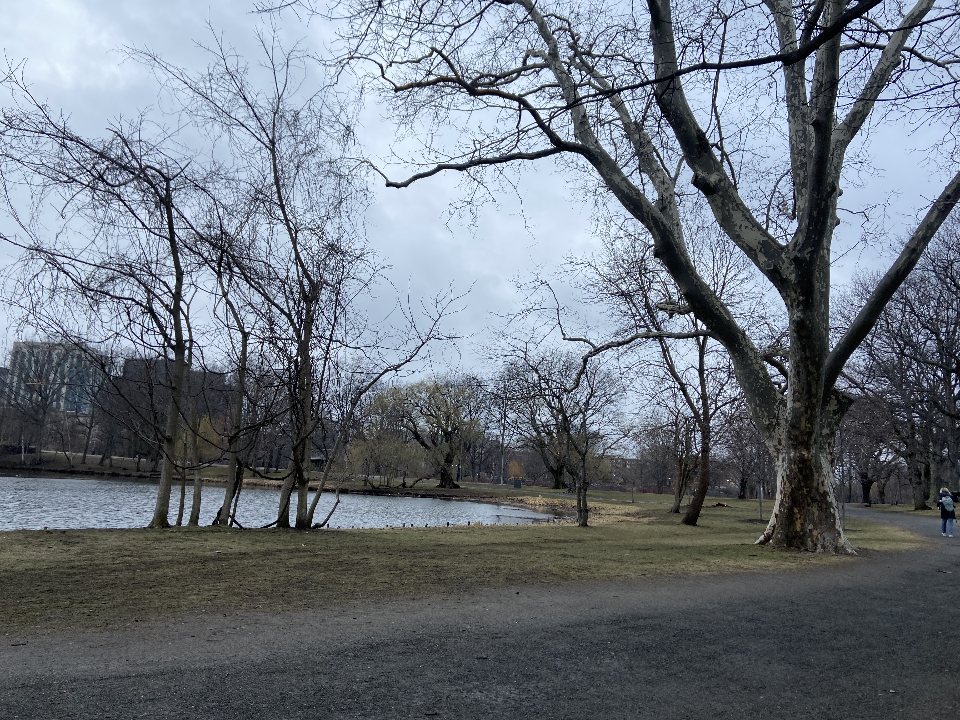
\includegraphics[width=0.7\textwidth]{report_imgs/00_original.png}
    \caption{Task 1: Static image displayed using \texttt{cv::imshow}.}
\end{figure}

%------------------------------------------------------------
\subsection*{Task 2 -- Live Color Video}
%------------------------------------------------------------

\begin{figure}[H]
    \centering
    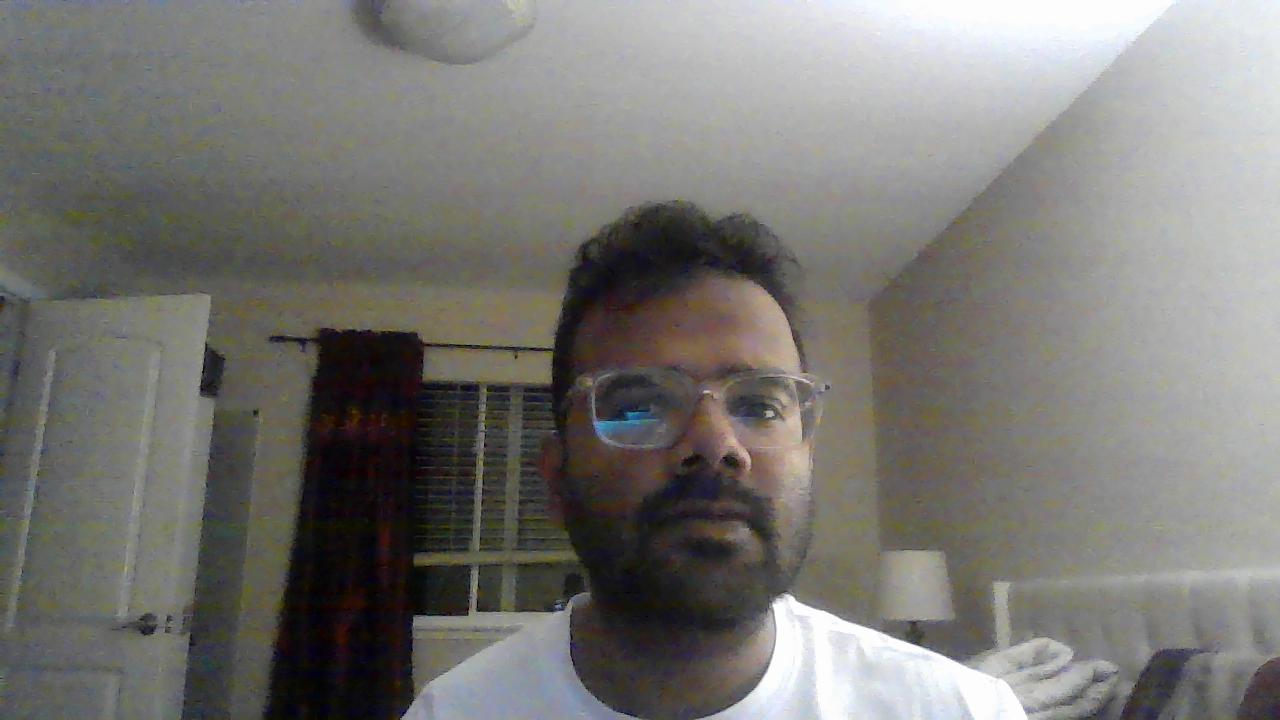
\includegraphics[width=0.7\textwidth]{report_imgs/img2.png}
    \caption{Task 2: Live color video frame from the webcam displayed using
    \texttt{cv::imshow}.}
\end{figure}

%------------------------------------------------------------
\subsection*{Task 3 -- OpenCV Greyscale}
%------------------------------------------------------------

\begin{figure}[H]
    \centering
    \begin{subfigure}[b]{0.48\textwidth}
        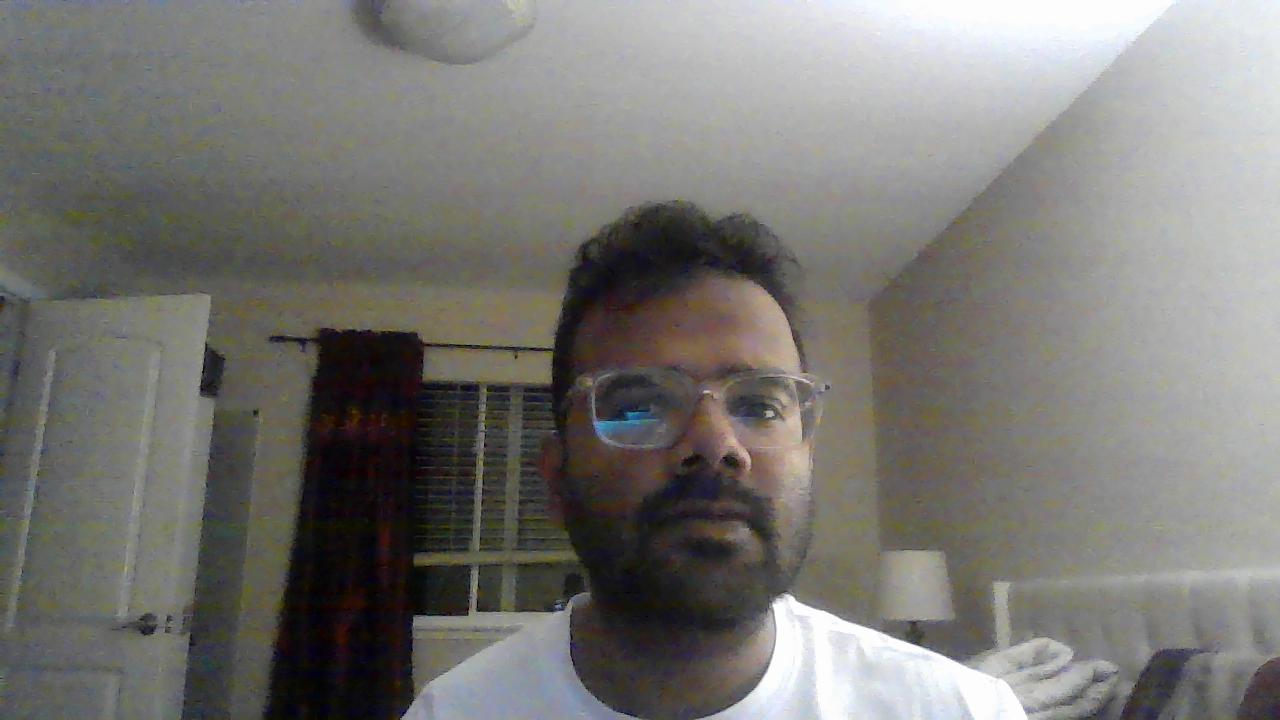
\includegraphics[width=\textwidth]{report_imgs/img2.png}
        \caption{Original color frame}
    \end{subfigure}
    \hfill
    \begin{subfigure}[b]{0.48\textwidth}
        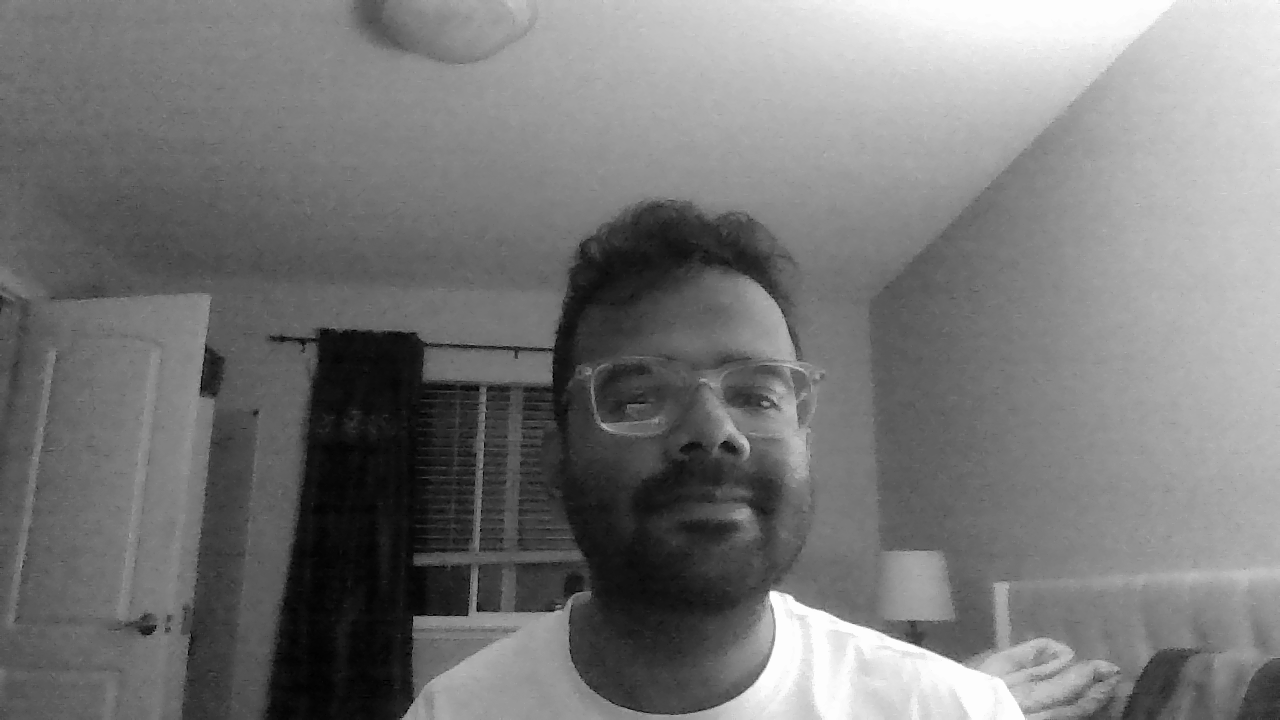
\includegraphics[width=\textwidth]{report_imgs/img3.png}
        \caption{\texttt{cvtColor} greyscale output}
    \end{subfigure}
    \caption{Task 3: Standard greyscale using \texttt{cv::COLOR\_BGR2GRAY}.
    According to the OpenCV docs, it uses the formula
    $Y = 0.299R + 0.587G + 0.114B$, which comes from the ITU-R BT.601
    standard. Green gets the most weight because the human eye is most
    sensitive to green light.}
\end{figure}

%------------------------------------------------------------
\subsection*{Task 4 -- Custom Greyscale}
%------------------------------------------------------------

\begin{figure}[H]
    \centering
    \begin{subfigure}[b]{0.48\textwidth}
        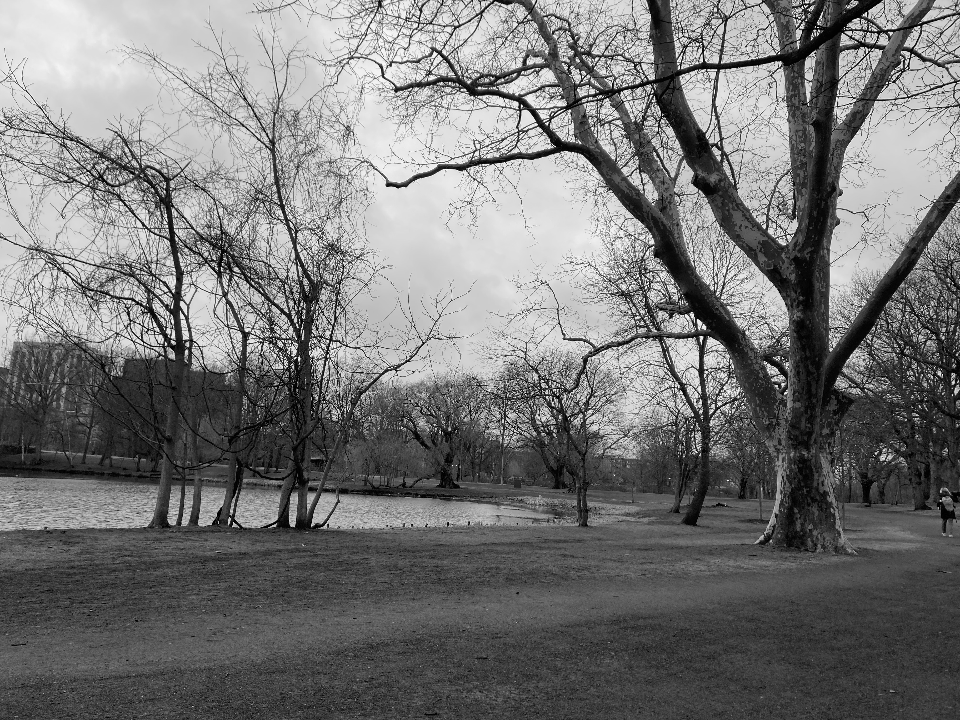
\includegraphics[width=\textwidth]{report_imgs/img1a_opencv_grey.png}
        \caption{OpenCV greyscale ($0.299R + 0.587G + 0.114B$)}
    \end{subfigure}
    \hfill
    \begin{subfigure}[b]{0.48\textwidth}
        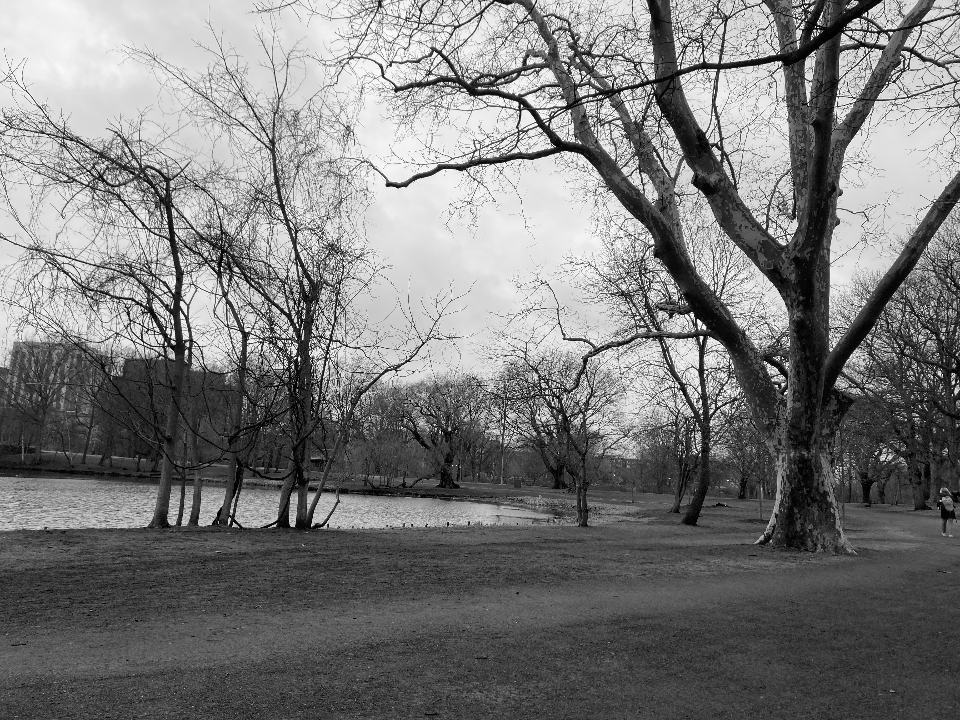
\includegraphics[width=\textwidth]{report_imgs/img2_custom_grey.png}
        \caption{Custom greyscale ($0.15R + 0.35G + 0.50B$)}
    \end{subfigure}
    \caption{Task 4: Custom greyscale with a blue-channel emphasis.
    We used weights $0.15R + 0.35G + 0.50B$ so blue is weighted about
    4 times more than in the standard formula. This makes warm-colored
    (red/orange) regions look darker and cool-colored (blue) regions look
    brighter compared to the OpenCV version. All three output channels
    are set to the same value so it is actually greyscale. Pixels are
    accessed using row pointers (\texttt{ptr<Vec3b>}).}
\end{figure}

%------------------------------------------------------------
\subsection*{Task 5 -- Sepia Tone}
%------------------------------------------------------------

\begin{figure}[H]
    \centering
    \begin{subfigure}[b]{0.48\textwidth}
        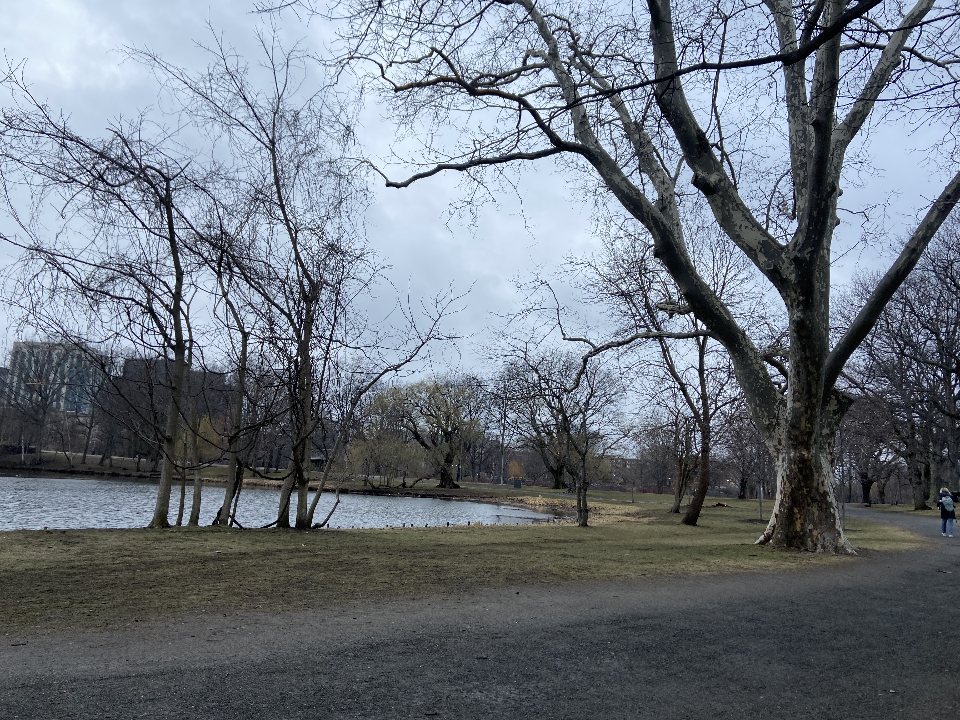
\includegraphics[width=\textwidth]{report_imgs/00_original.png}
        \caption{Original color frame}
    \end{subfigure}
    \hfill
    \begin{subfigure}[b]{0.48\textwidth}
        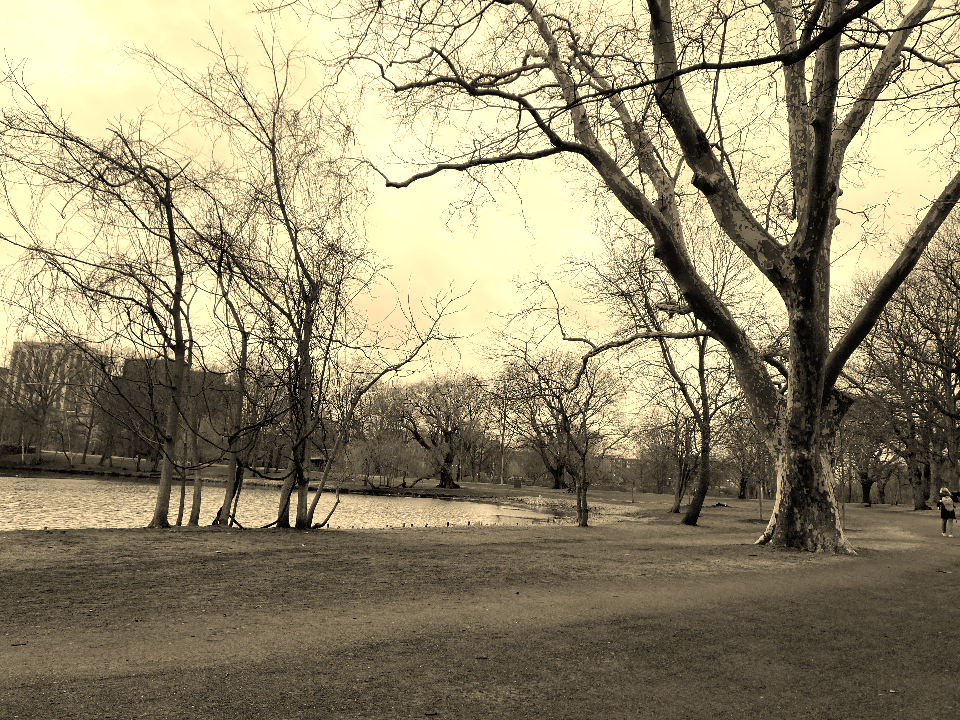
\includegraphics[width=\textwidth]{report_imgs/img3_sepia.png}
        \caption{Sepia filter output}
    \end{subfigure}
    \caption{Task 5: Sepia tone filter. Each output channel is a weighted
    combination of all three input channels:
    $B' = 0.272R + 0.534G + 0.131B$,
    $G' = 0.349R + 0.686G + 0.168B$,
    $R' = 0.393R + 0.769G + 0.189B$.
    To make sure we always use the original values, we read all three
    channels into float variables before writing anything. That way no
    output channel can accidentally influence another. We also clamp
    values to 255 since the red and green rows of coefficients sum
    to more than 1.}
\end{figure}

%------------------------------------------------------------
\subsection*{Task 6 -- 5x5 Gaussian Blur}
%------------------------------------------------------------

\begin{figure}[H]
    \centering
    \begin{subfigure}[b]{0.48\textwidth}
        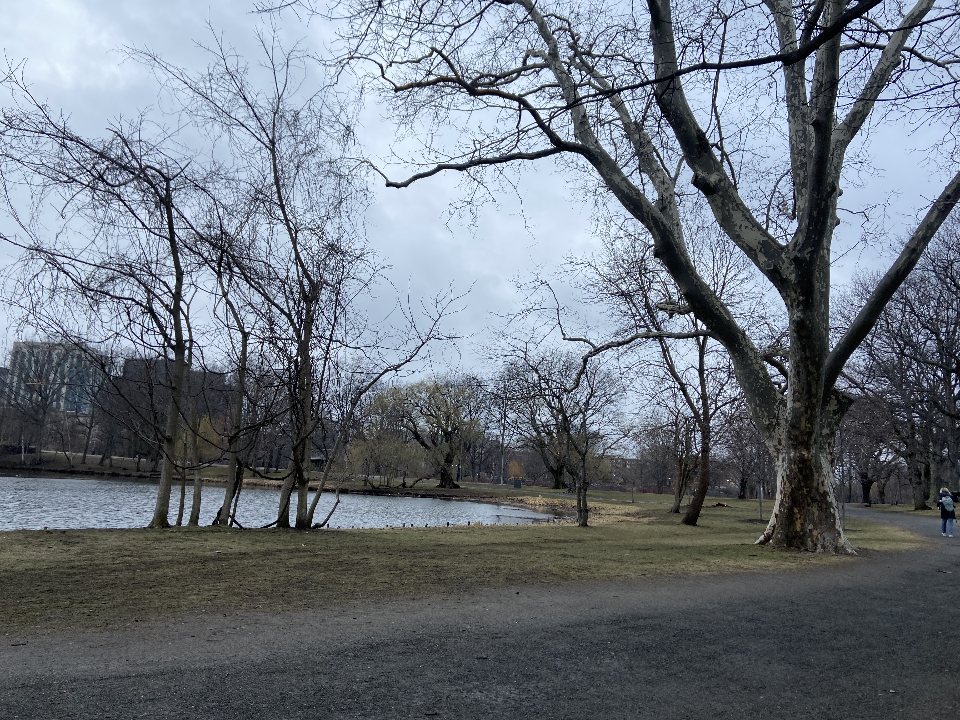
\includegraphics[width=\textwidth]{report_imgs/00_original.png}
        \caption{Original color frame}
    \end{subfigure}
    \hfill
    \begin{subfigure}[b]{0.48\textwidth}
        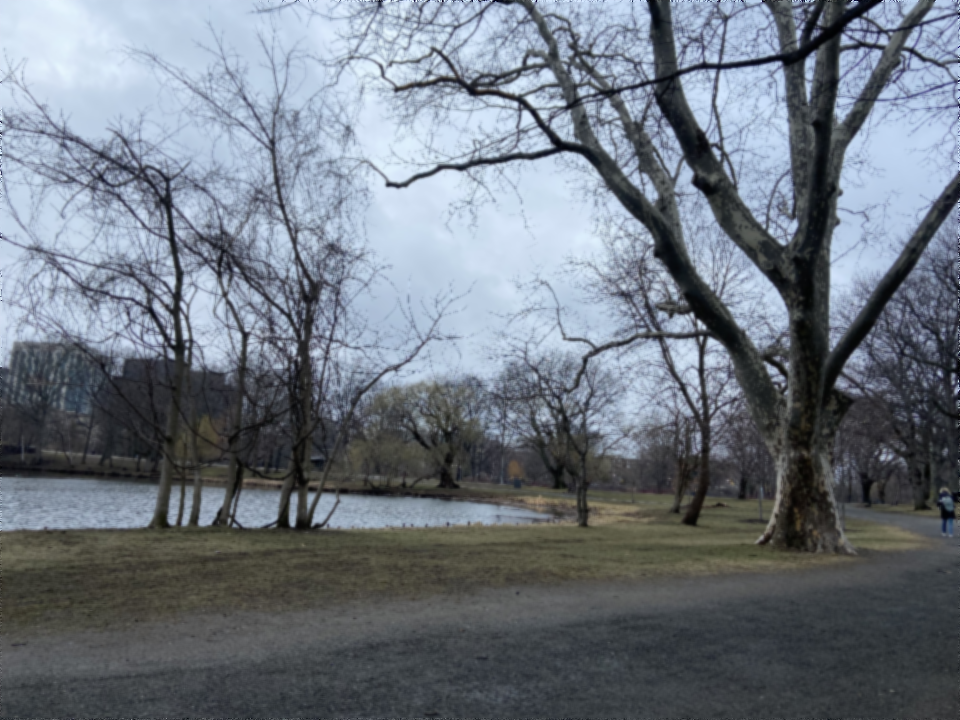
\includegraphics[width=\textwidth]{report_imgs/img4b_blur.png}
        \caption{After \texttt{blur5x5\_2}}
    \end{subfigure}
    \caption{Task 6: 5x5 Gaussian blur applied to each color channel separately.
    The kernel used is $[1\;2\;4\;2\;1;\;2\;4\;8\;4\;2;\;4\;8\;16\;8\;4;\;
    2\;4\;8\;4\;2;\;1\;2\;4\;2\;1]$ with a sum of 100.}
\end{figure}

\subsubsection*{Timing Comparison (960x720 image, average of 5 runs)}

\begin{table}[H]
\centering
\begin{tabular}{lll}
\toprule
\textbf{Function} & \textbf{Avg. time} & \textbf{Method} \\
\midrule
\texttt{blur5x5\_1} & 16.01 ms & Nested loop with \texttt{.at<>} \\
\texttt{blur5x5\_2} & 3.81 ms  & Separable passes and row pointers \\
\bottomrule
\end{tabular}
\caption{\texttt{blur5x5\_2} is about 4x faster for two reasons.
First, we split the 2D filter into a horizontal pass followed by a vertical
pass using the 1D kernel $[1\;2\;4\;2\;1]$. This cuts operations per pixel
from 25 down to 10. Second, we access pixels through row pointers
(\texttt{ptr<Vec3b>}) instead of \texttt{.at<>}, which avoids
bounds-checking on every access.}
\end{table}

%------------------------------------------------------------
\subsection*{Tasks 7 and 8 -- Sobel Filters and Gradient Magnitude}
%------------------------------------------------------------

\begin{figure}[H]
    \centering
    \begin{subfigure}[b]{0.48\textwidth}
        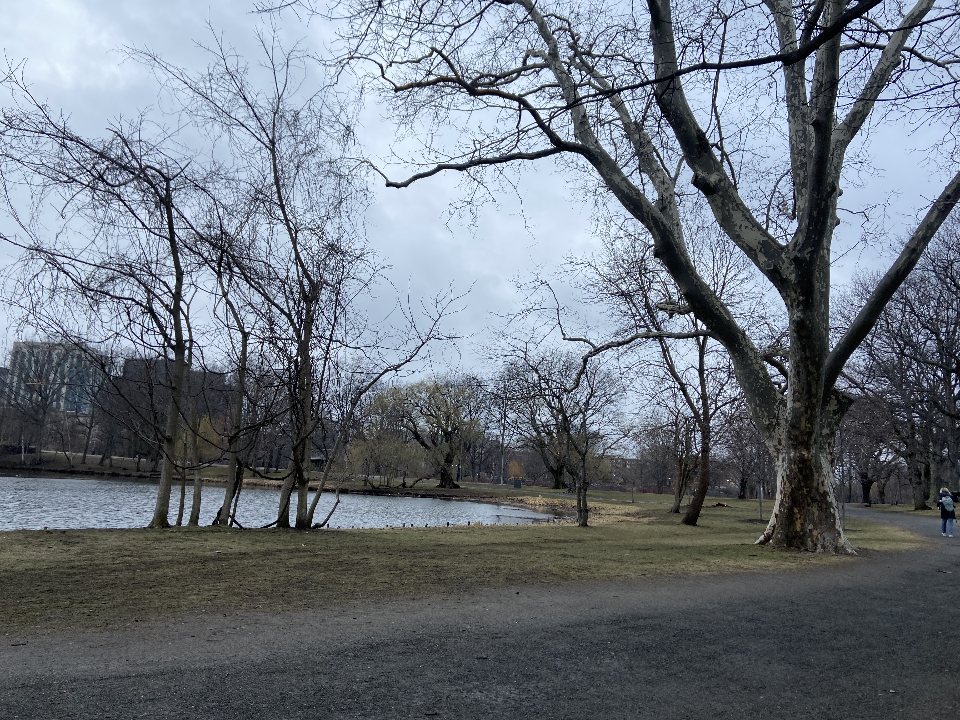
\includegraphics[width=\textwidth]{report_imgs/00_original.png}
        \caption{Original}
    \end{subfigure}
    \hfill
    \begin{subfigure}[b]{0.48\textwidth}
        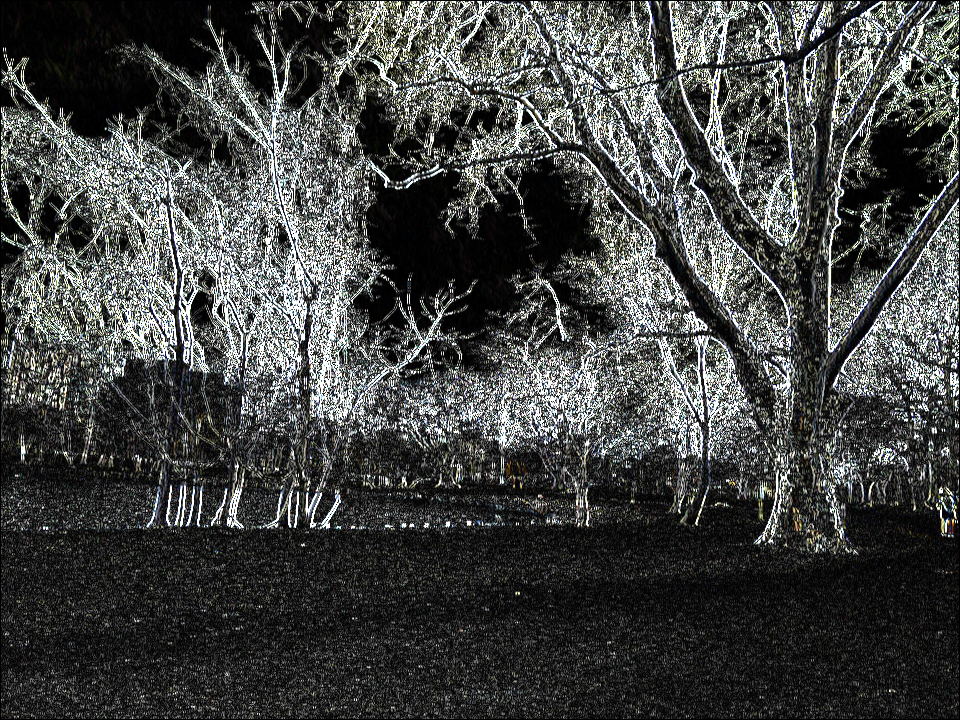
\includegraphics[width=\textwidth]{report_imgs/img5a_sobelX.png}
        \caption{Sobel X (absolute value shown)}
    \end{subfigure}

    \vspace{0.5em}

    \begin{subfigure}[b]{0.48\textwidth}
        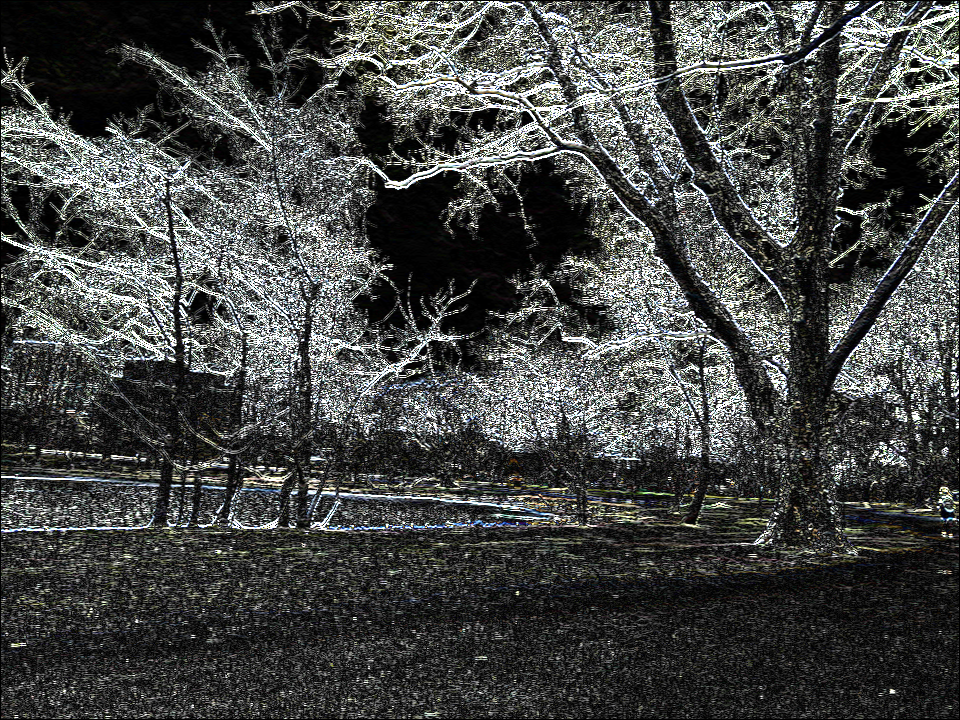
\includegraphics[width=\textwidth]{report_imgs/img5b_sobelY.png}
        \caption{Sobel Y (absolute value shown)}
    \end{subfigure}
    \hfill
    \begin{subfigure}[b]{0.48\textwidth}
        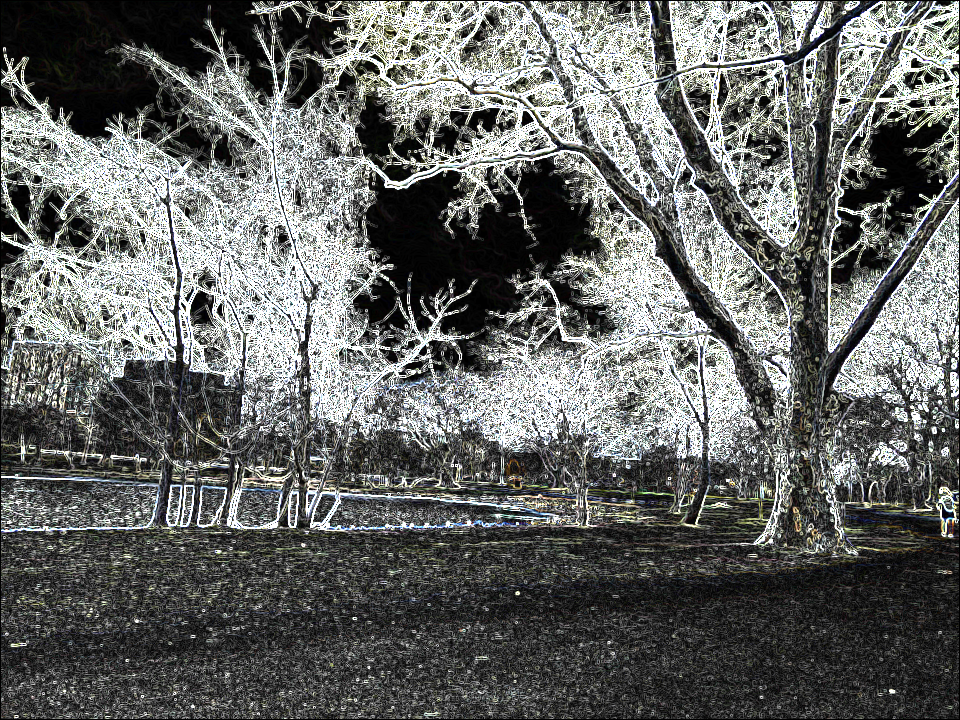
\includegraphics[width=\textwidth]{report_imgs/img5c_magnitude.png}
        \caption{Gradient magnitude}
    \end{subfigure}
    \caption{Tasks 7 and 8: Sobel edge detection and gradient magnitude.
    Sobel X picks up vertical edges (left-to-right intensity changes) using
    the separable filters $[-1\;0\;1]$ horizontal then $[1\;2\;1]$ vertical,
    with positive values meaning a right-going gradient.
    Sobel Y picks up horizontal edges using $[1\;2\;1]$ horizontal then
    $[1\;0\;-1]$ vertical, with positive values meaning an upward gradient.
    Both functions output \texttt{CV\_16SC3} (signed short) because the
    values can be negative and can go up to 1020 in magnitude.
    We keep a separate variable for display and use \texttt{convertScaleAbs}
    only for that, not for the filter output itself.
    The magnitude image combines both directions:
    $M = \sqrt{s_x^2 + s_y^2}$ per channel, clamped to 255.}
\end{figure}

%------------------------------------------------------------
\subsection*{Task 9 -- Blur and Quantize}
%------------------------------------------------------------

\begin{figure}[H]
    \centering
    \begin{subfigure}[b]{0.48\textwidth}
        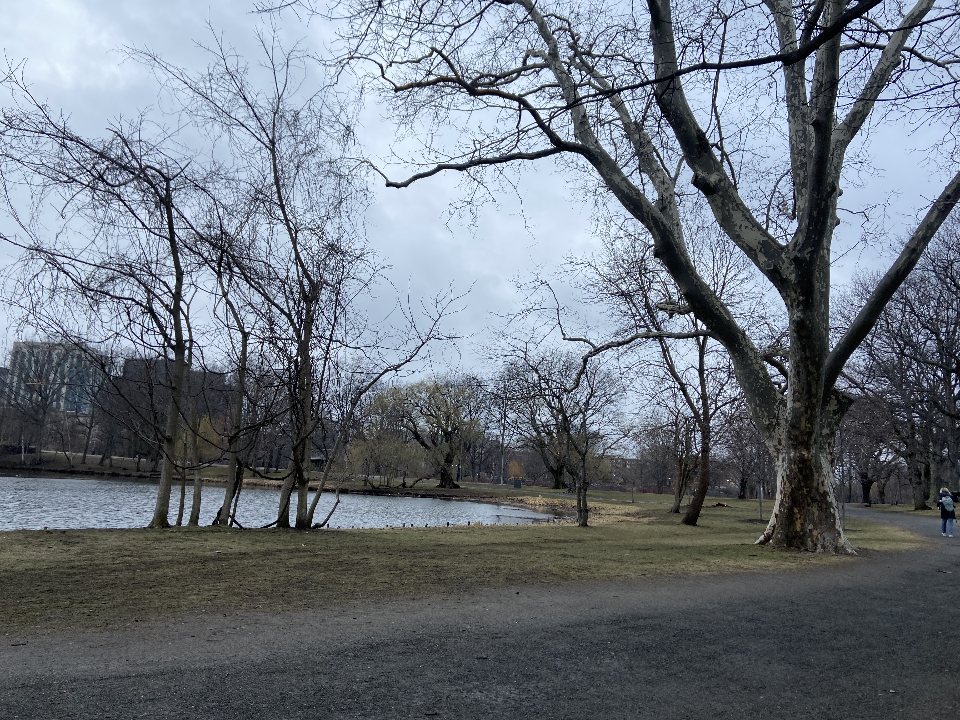
\includegraphics[width=\textwidth]{report_imgs/00_original.png}
        \caption{Original color frame}
    \end{subfigure}
    \hfill
    \begin{subfigure}[b]{0.48\textwidth}
        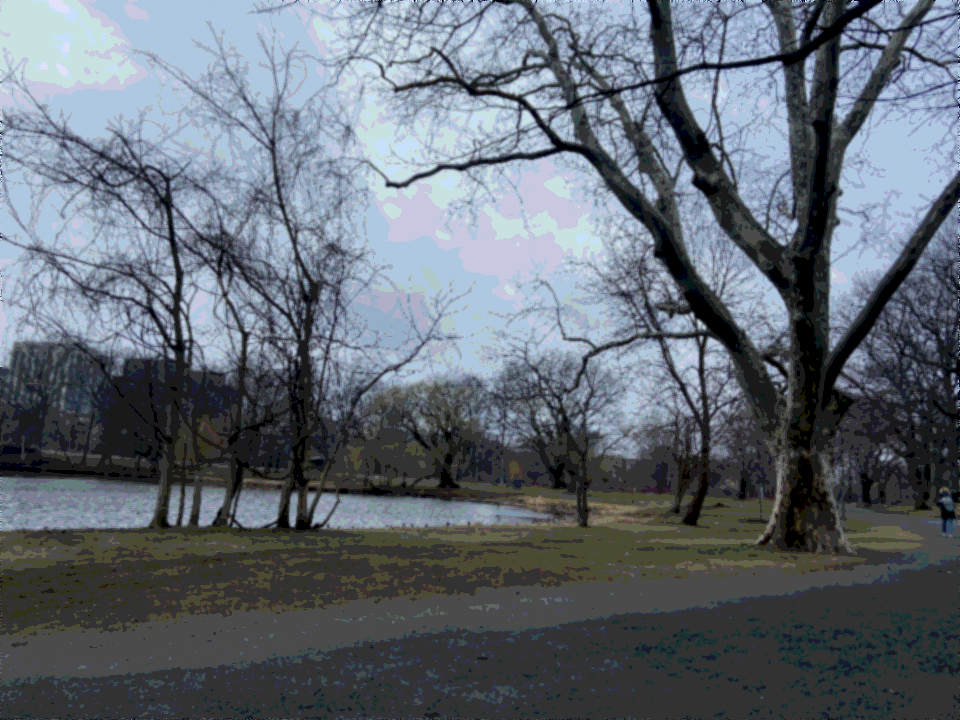
\includegraphics[width=\textwidth]{report_imgs/img6_blurquantize.png}
        \caption{\texttt{blurQuantize} with 10 levels}
    \end{subfigure}
    \caption{Task 9: Blur then quantize. We first run \texttt{blur5x5\_2}
    to smooth the image, then snap each channel to the nearest bucket value:
    $\text{bucket} = 255 / \text{levels}$, $x_t = \lfloor x / \text{bucket} \rfloor$,
    $x_f = x_t \times \text{bucket}$.
    With 10 levels per channel the image can have at most $10^3 = 1000$
    distinct colors, which gives a cartoon or poster look. Blurring first
    helps because without it the quantization looks noisy.}
\end{figure}

%------------------------------------------------------------
\subsection*{Task 10 -- Face Detection}
%------------------------------------------------------------

\begin{figure}[H]
    \centering
    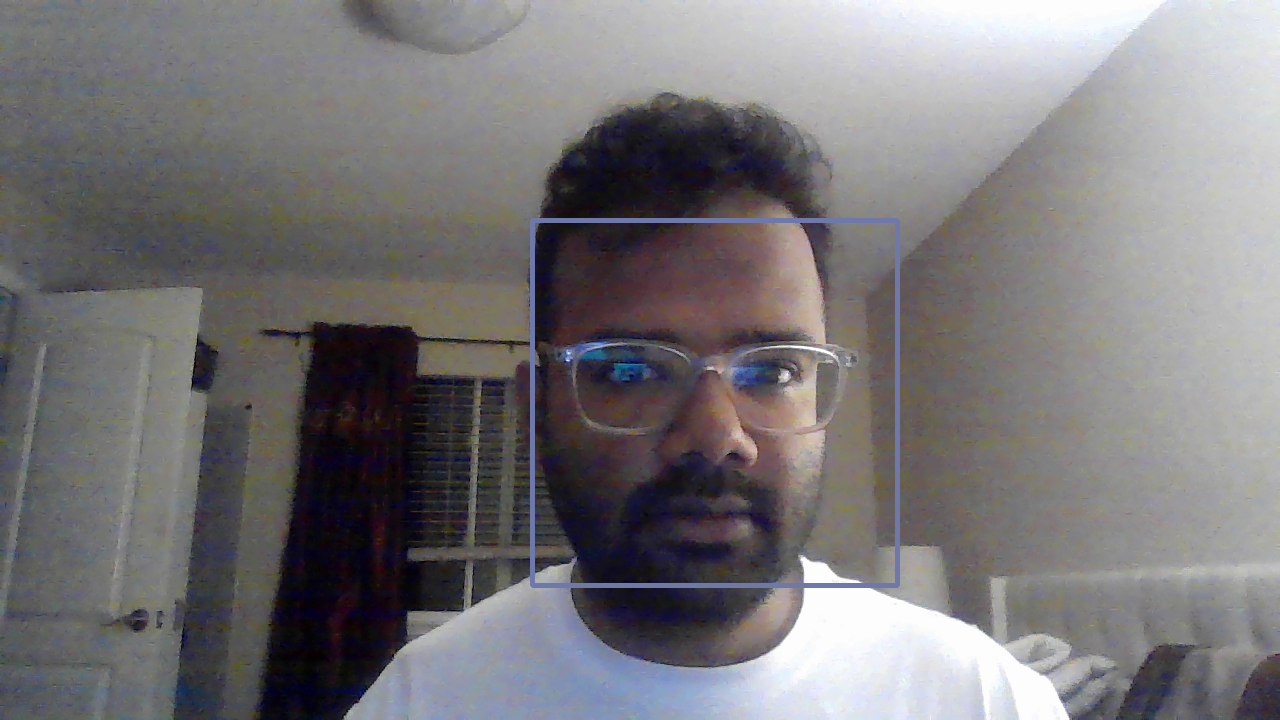
\includegraphics[width=0.7\textwidth]{report_imgs/img10_after_fd.png}
    \caption{Task 10: Haar cascade face detection. Detected faces are highlighted
    with bounding boxes drawn using \texttt{drawBoxes}. The cascade classifier
    runs on a greyscale version of the frame and the boxes are overlaid on the
    original color frame.}
\end{figure}

%------------------------------------------------------------
\subsection*{Task 11 -- Depth Estimation}
%------------------------------------------------------------

\begin{figure}[H]
    \centering
    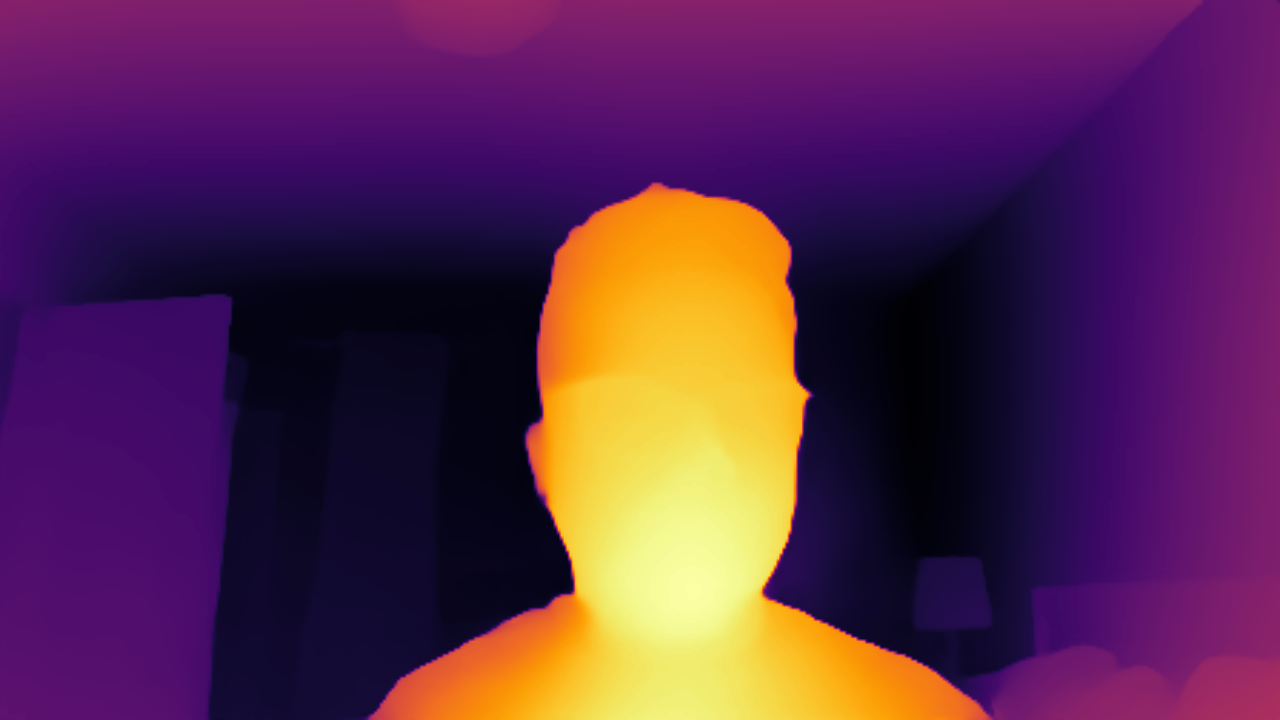
\includegraphics[width=0.7\textwidth]{report_imgs/img11_depth.png}
    \caption{Task 11: Depth Anything V2 depth map rendered with the INFERNO
    colormap. Brighter regions are closer to the camera; darker regions are
    farther away.}
\end{figure}

\begin{figure}[H]
    \centering
    \begin{subfigure}[b]{0.48\textwidth}
        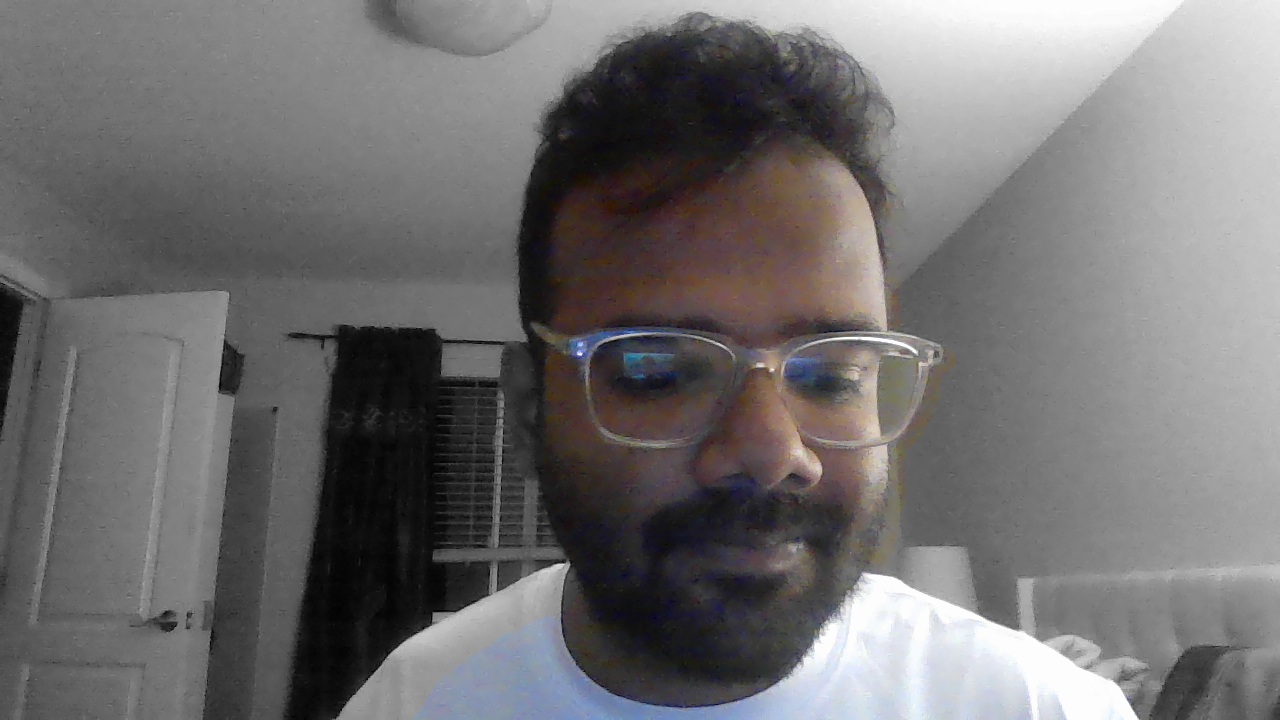
\includegraphics[width=\textwidth]{report_imgs/img11_close_color.png}
        \caption{Close foreground stays in color}
    \end{subfigure}
    \hfill
    \begin{subfigure}[b]{0.48\textwidth}
        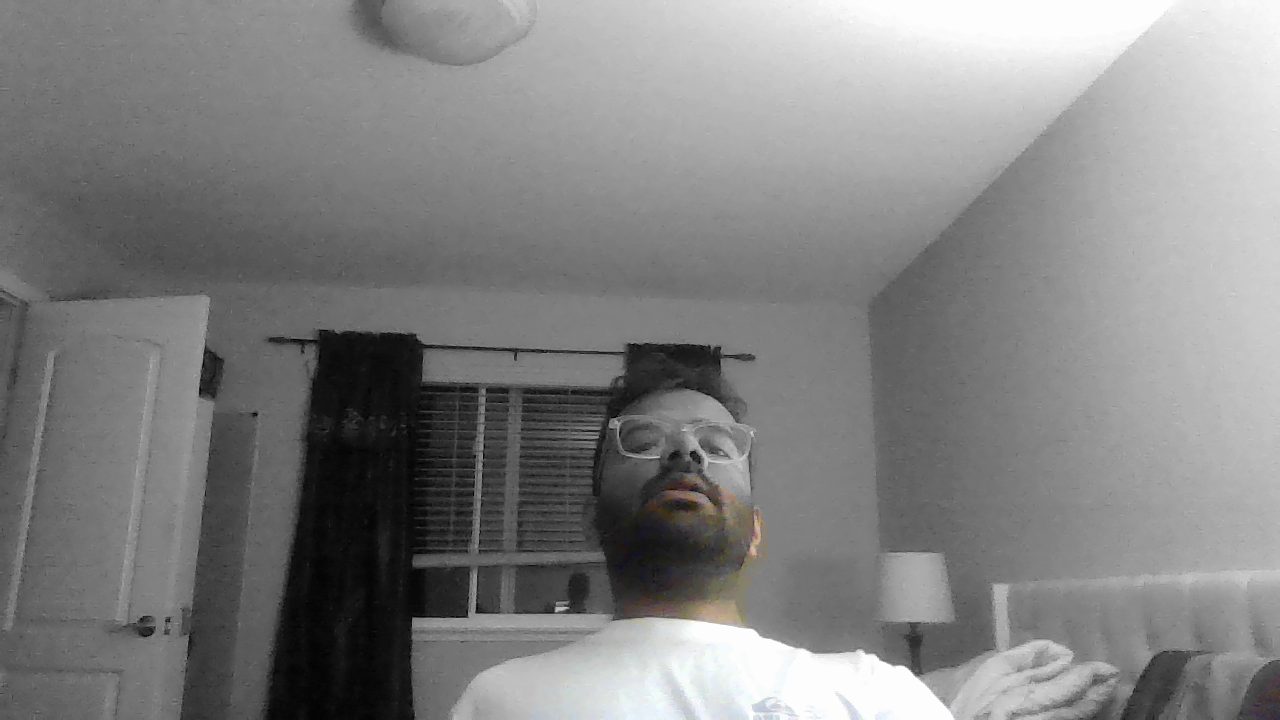
\includegraphics[width=\textwidth]{report_imgs/img11_far_gray.png}
        \caption{Far background converted to greyscale}
    \end{subfigure}
    \caption{Task 11 creative filter: depth-based background greyscale.
    Pixels with depth above the threshold (close objects) remain in color
    while pixels below the threshold (far background) are converted to
    greyscale.}
\end{figure}

%------------------------------------------------------------
\subsection*{Task 12 -- Custom Effects}
%------------------------------------------------------------

We chose three effects that each meet one of the requirements:

\begin{description}
    \item[Color Negative (\texttt{n}, pixel-wise):] Inverts every channel
        value with $\text{dst}[c] = 255 - \text{src}[c]$. No neighbors
        needed.
    \item[Emboss (\texttt{e}, area-based):] Takes the signed Sobel X and Y
        outputs from Tasks 7 and 8, computes their dot product with a light
        direction of $(0.7071,\,0.7071)$, averages across the three channels,
        then adds 128 so flat areas map to mid-grey.
    \item[Depth Fog (\texttt{o}, uses depth):] Uses the DA2 depth map to
        add exponential fog. The formula is $\text{fog} = 1 - e^{-k \cdot d}$
        where $d = 1 - \text{depth}/255$. Close objects stay clear and far
        objects fade toward a grey fog color.
\end{description}

\begin{figure}[H]
    \centering
    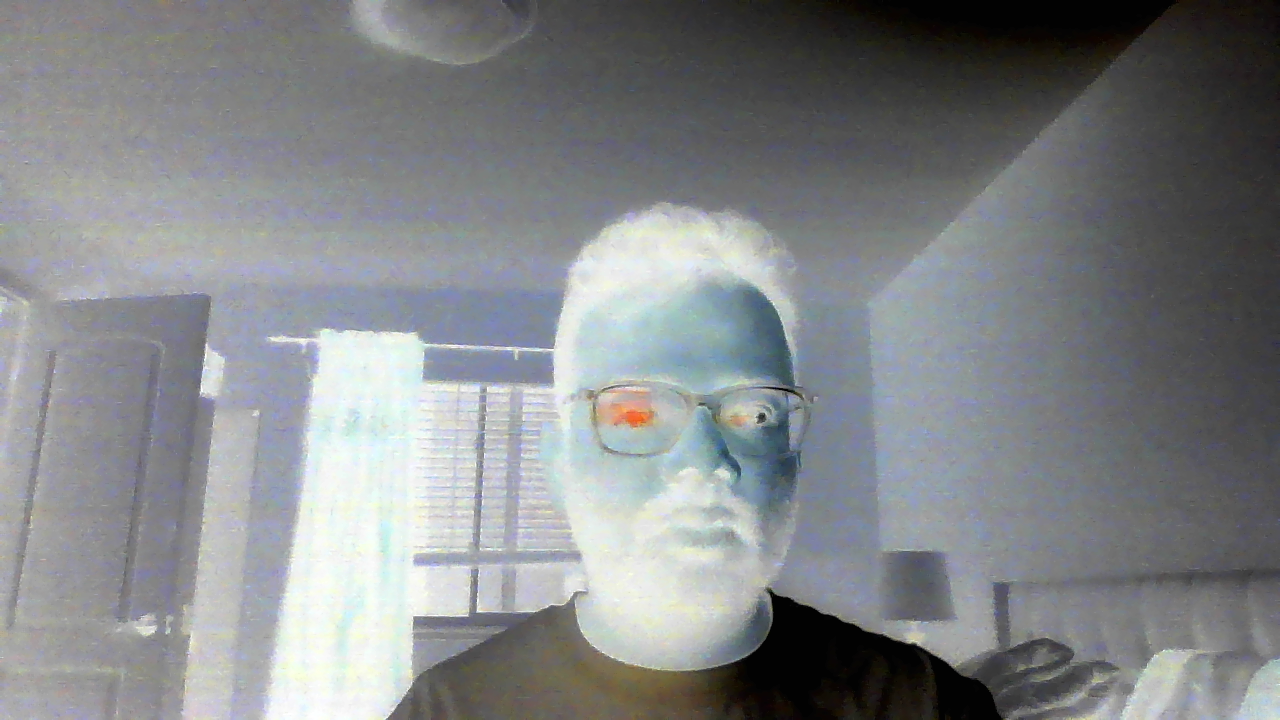
\includegraphics[width=0.7\textwidth]{report_imgs/img12a_negative.png}
    \caption{Task 12a: Color negative. Each channel is inverted with
    $\text{dst}[c] = 255 - \text{src}[c]$.}
\end{figure}

\begin{figure}[H]
    \centering
    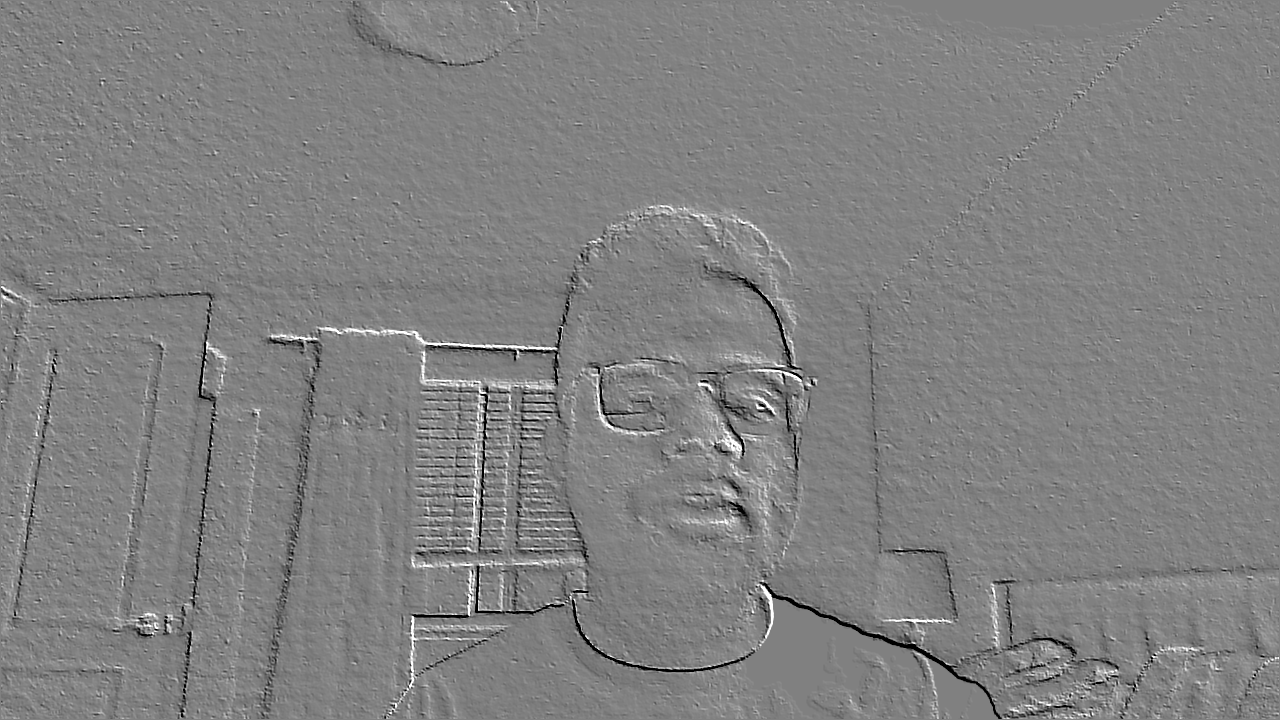
\includegraphics[width=0.7\textwidth]{report_imgs/img12b_emboss.png}
    \caption{Task 12b: Emboss effect. Sobel X and Y outputs are combined
    with a light direction of $(0.7071,\,0.7071)$ and offset by 128 so
    flat areas map to mid-grey.}
\end{figure}

\begin{figure}[H]
    \centering
    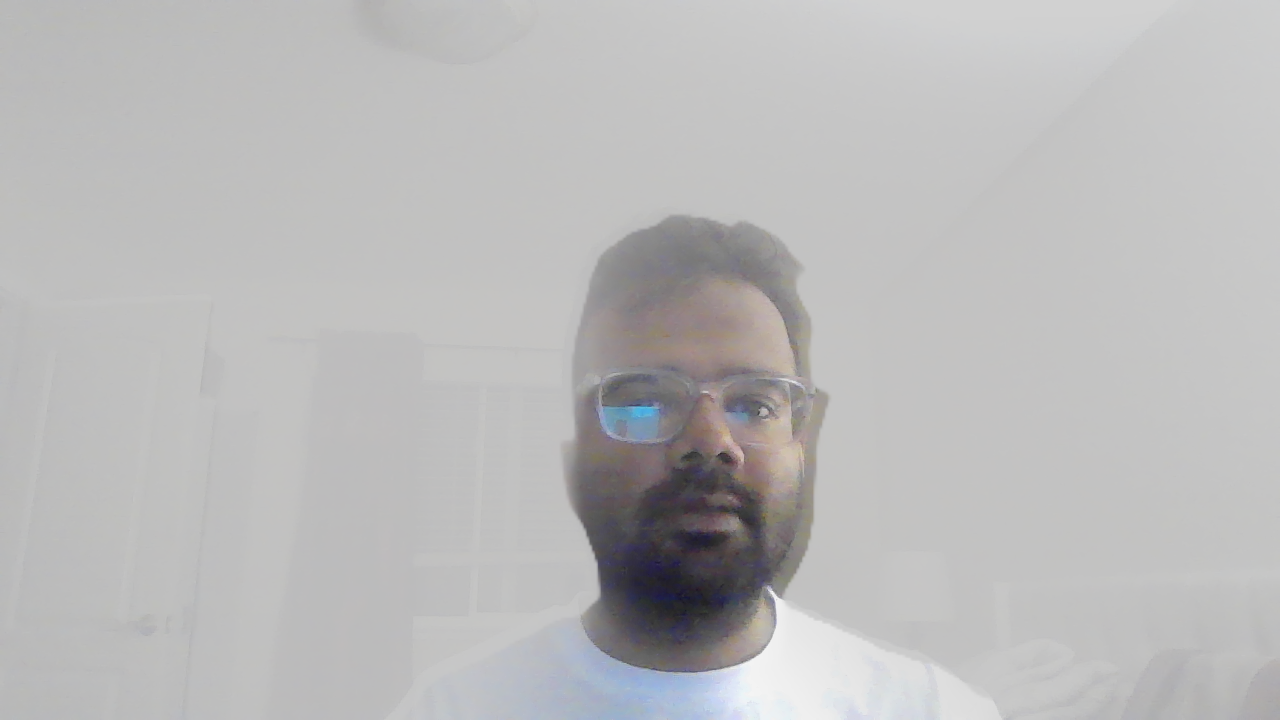
\includegraphics[width=0.7\textwidth]{report_imgs/img12c_depthfog.png}
    \caption{Task 12c: Depth-based exponential fog. Close objects remain
    clear while far objects fade toward a grey fog color using
    $\text{fog} = 1 - e^{-k \cdot d}$ where $d = 1 - \text{depth}/255$.}
\end{figure}

% ============================================================
\section*{Extensions}
% ============================================================

We did not pursue formal extensions beyond the required tasks. The depth fog
filter (Task 12c) builds directly on Task 11 using a physically-based model
for atmospheric scattering rather than a simple depth threshold, so it could
count as a small extension of that task.

% ============================================================
\section*{Reflection}
% ============================================================

\begin{itemize}
    \item Working at the pixel level with \texttt{cv::Mat} made us realize
        that images are just arrays of numbers, and most of what makes a
        filter look good is a careful choice of weights or thresholds applied
        to those numbers.
    \item Writing two versions of the blur filter and timing them taught us
        that algorithmic decisions matter more than we expected. Switching from
        \texttt{.at<>} to row pointers and using separable 1D passes instead
        of a full 2D kernel gave a 4x speedup on the same hardware.
    \item The Sobel filter was initially confusing because Sobel X detects
        horizontal changes but shows vertical edges in the output. Reasoning
        through that helped us understand the relationship between the direction
        of a gradient and the orientation of edges.
    \item Using signed 16-bit output for the Sobel functions was something we
        had not thought about before. Without it, negative gradient values
        would be clipped silently and the results would be wrong.
    \item Integrating Depth Anything V2 through the ONNX runtime showed us
        how modern deep networks can fit into a classical CV pipeline. Having
        per-pixel depth information opens up filter ideas that are not possible
        with just the RGB values.
    \item Face detection with a Haar cascade was fast and surprisingly easy
        to wire in, which made us curious about how much more accurate but
        slower methods like deep learning detectors compare in practice.
    \item Overall this project changed how we look at filters in tools like
        Photoshop or Instagram. What seemed like magic before is now a pretty
        understandable sequence of per-pixel math operations.
\end{itemize}

% ============================================================
\section*{Acknowledgements}
% ============================================================

\begin{itemize}
    \item OpenCV documentation (\url{https://docs.opencv.org/4.x/}) for
        the \texttt{cvtColor} channel weights and pixel access patterns.
    \item Shriman Raghav Srinivasan implemented Tasks 4 through 9, including
        the custom greyscale, sepia tone, both blur implementations, Sobel X
        and Y filters, gradient magnitude, and blur-and-quantize functions in
        \texttt{filter.cpp} and \texttt{filter.h}.
    \item Shyam Sreenivasan handled initial project setup including environment
        configuration, package installation, and validation of dependencies
        (OpenCV, ONNX runtime, Depth Anything V2). He also implemented Tasks 1
        through 3 and Tasks 10 through 12 (face detection, Depth Anything V2,
        and the three custom effects).
    \item We used Claude (Anthropic) as an AI assistant to help set up the
        initial code structure and for debugging during development.
\end{itemize}

\end{document}
